\documentclass{ctexart}
\usepackage{amsmath}
\usepackage{float}
\usepackage{amssymb}
\usepackage{graphicx}
\usepackage{gbt7714}
\usepackage{pifont}
\usepackage{wrapfig}
\usepackage{multirow}
\usepackage{subfig}
\ctexset{
    % 修改 section。
    section={   
        name={,、},
        number={\chinese{section}}
    }
}

\title{在气垫导轨上测量瞬时速度与加速度}
\author{陆知辰-10225301478}
\date{\today}
\graphicspath{{figure/}}

\begin{document}

\begin{titlepage}
  \centering
  % 插入图片
  
\includegraphics[width=0.5\textwidth]{ecnu.png}
  
  % 空行用于调整标题位置
  \vspace*{\baselineskip}
  
  % 标题
  \Huge\textbf{物\quad 理\quad 实\quad 验 \quad (三)}
  % 空行用于调整标题和其他信息之间的间距
  \vspace*{0.3\baselineskip}
  
  % 具体实验名称
  \huge 在气垫导轨测量瞬时速度与加速度
  
  % 空行用于调整时间和其他信息之间的间距
  \vspace*{2\baselineskip}
  
  % 时间
  \large 时间:\today
  
  % 空行用于调整时间和其他信息之间的间距
  \vspace*{\baselineskip}
  
  % 创作人
  \large 创作人:陆知辰
  
  % 空行用于调整创作人和学号之间的间距
  \vspace*{\baselineskip}
  
  % 学号
  \large 学号:10225301478
  
\end{titlepage}
\newpage
\tableofcontents
\newpage
\section{实验摘要}
  \subsection{实验概要}
  气垫导轨为力学试验提供了一维几乎无摩擦的系统,在气垫导轨上研究物体的一维运动能够更加简洁方便。
  本实验采用气垫导轨验证匀加速直线运动的公式和牛顿第一定律。
  \subsection{实验目的}
  1.\quad 掌握光点计时器的使用方法,能够用光电计时器测量时间、速度、加速度。

  2.\quad 了解气垫导轨的特点,掌握气垫导轨的调节方法。
  
  3.\quad 学会使用图解法设计实验、验证物理规律。

\section{实验原理}
气垫导轨表面具有规则排列的小孔,如图\ref{jiegou}所示,
在与气源连通后,从小孔处将会有压缩空气喷出,从而在导轨和放置于导轨上的滑块之间形成一层很薄的“气垫”,
使滑块漂浮在气垫上。此时,滑块在气垫上的运动仅受到很小的空气黏性摩擦阻力的作用,可以近似认为是无摩擦运动。
将已调至水平的气垫导轨一端垫上垫块,便得到一个较为理想的平直光滑斜面,
其示意图如图\ref{jiegou}所示。

\begin{figure}[H]
  \centering
  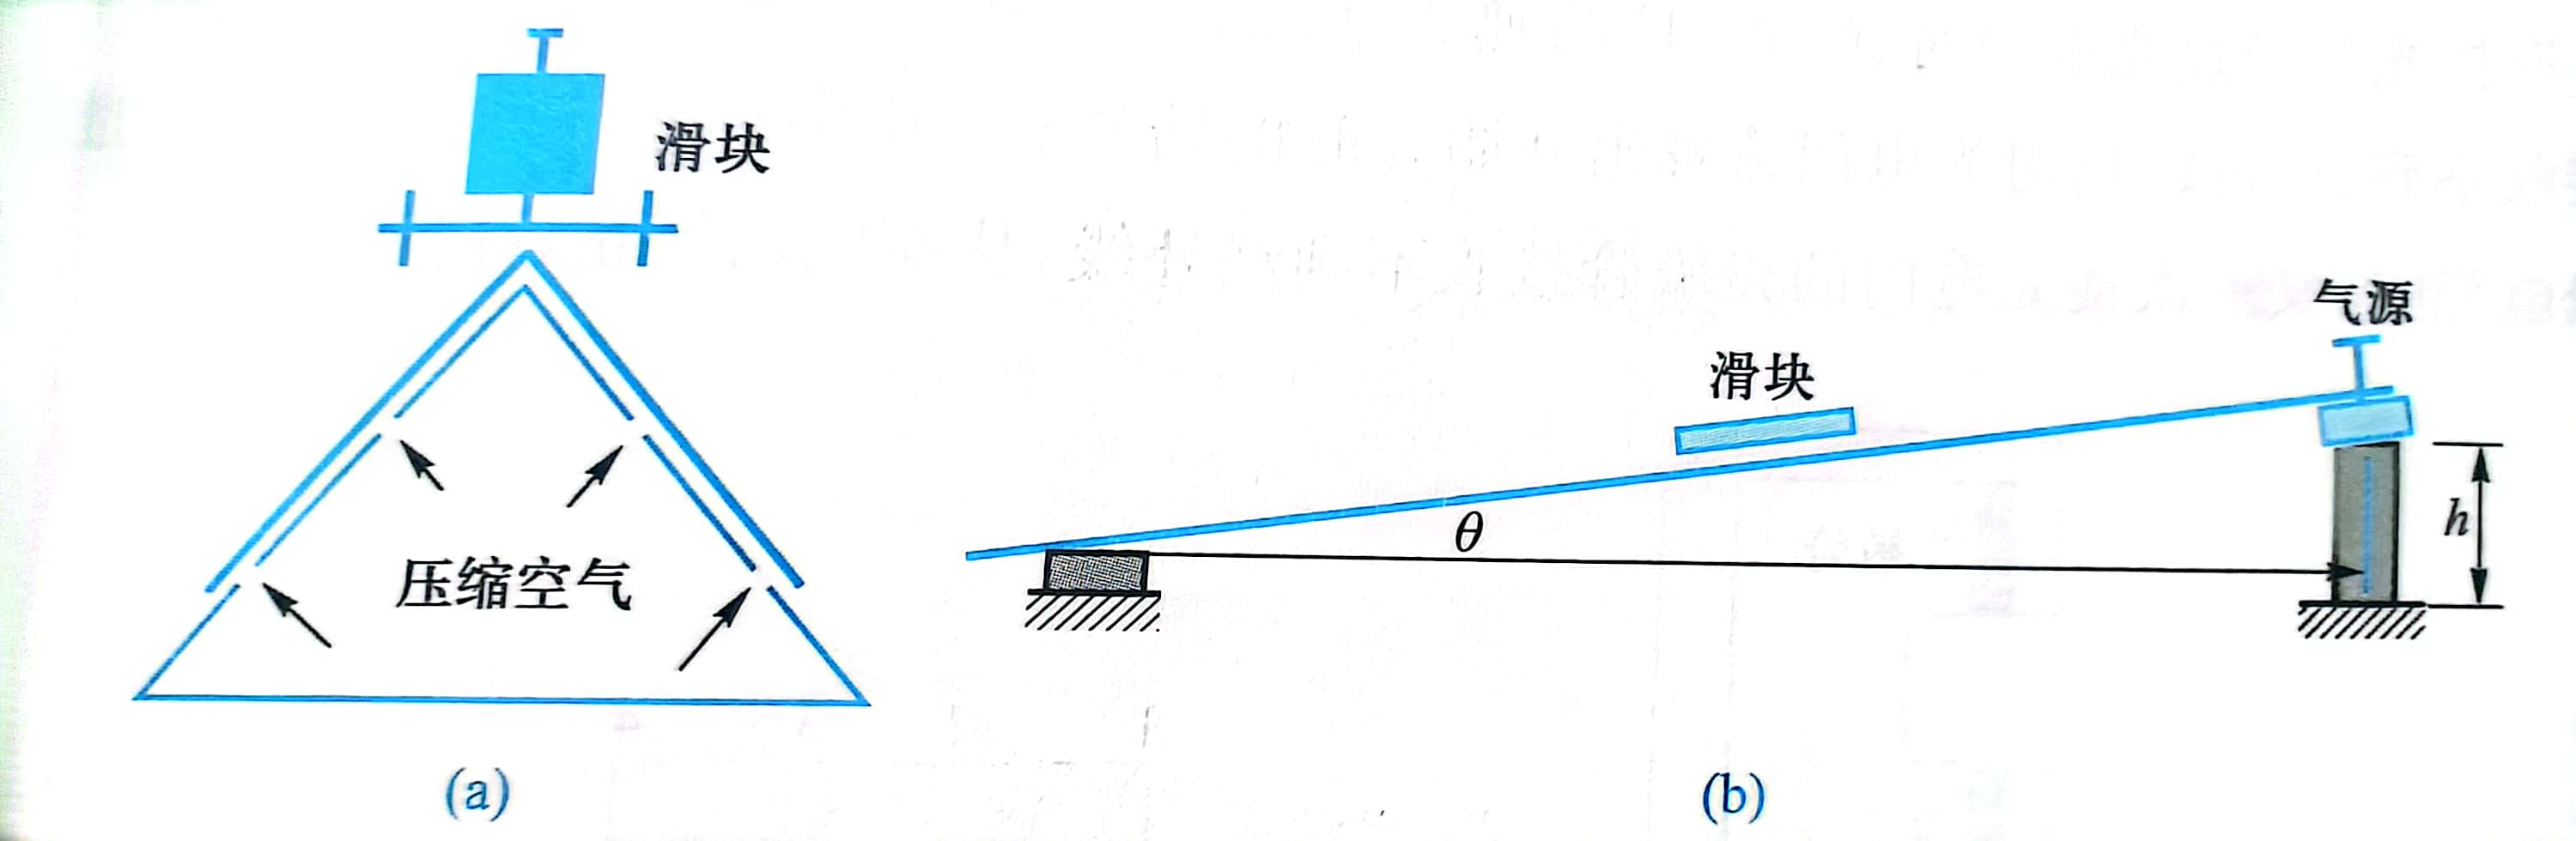
\includegraphics[height=0.2\textheight,width=0.9\textwidth]{jiegou.jpg}
  \caption{气垫导轨结构展示}\label{jiegou}
\end{figure}

在忽略空气摩擦阻力的情况下,滑块在重力沿斜面的分力作用下作匀加速直线运动,该运动由如下三个基本公式描述:

\begin{equation}
  v = v_{0} + at
\end{equation}
\begin{equation}
  s = v_{0}t + \frac{1}{2} at^{2}
\end{equation}
\begin{equation}\label{v2}
  v^{2} = v_{0}^{2} + 2as
\end{equation}

式中$v_{0}$和$v$分别为物体在$t=0$和$t=1$时刻的瞬时速度,$s$为物体在$t$时间内运动的距离,$a$为物体的加速度。
在气垫导轨所组成的斜面上,滑块下滑时的加速度$a$和重力加速度$g$之间关系为

\begin{equation}\label{jiasudu}
  a = g\sin\theta = g\frac{h}{L}
\end{equation}

式中$\theta$为气垫导轨的倾角,$h$为导轨调平后一端垫起的高度,即垫块的厚度,$L$为气
垫导轨两端底脚螺丝之间斜面部分的长度。

牛顿第一定律指出,一切物体总保持匀速直线运动状态或静止状态,除非作用在它上面的力迫使它改变这种状态,
由式\ref{jiasudu}可知,在h=0时,滑块的加速度a=0.
在实验中可通过测量a-h曲线,线性外推,从而验证在h=0时,a是否为0。
若a=0,说明导轨水平时,物体不受外力作用情况下会保持原来的匀速直线运动状态,从而可以验证牛顿第一定律。

\section{实验装置器材介绍}
气垫导轨以及气源、滑块以及U型挡光片、光电计时系统、游标卡尺、垫块等。

\section{实验内容及实验步骤}
  \subsection{节光电计时系统,使其正常工作}
  
  \begin{figure}[H]
    \centering
    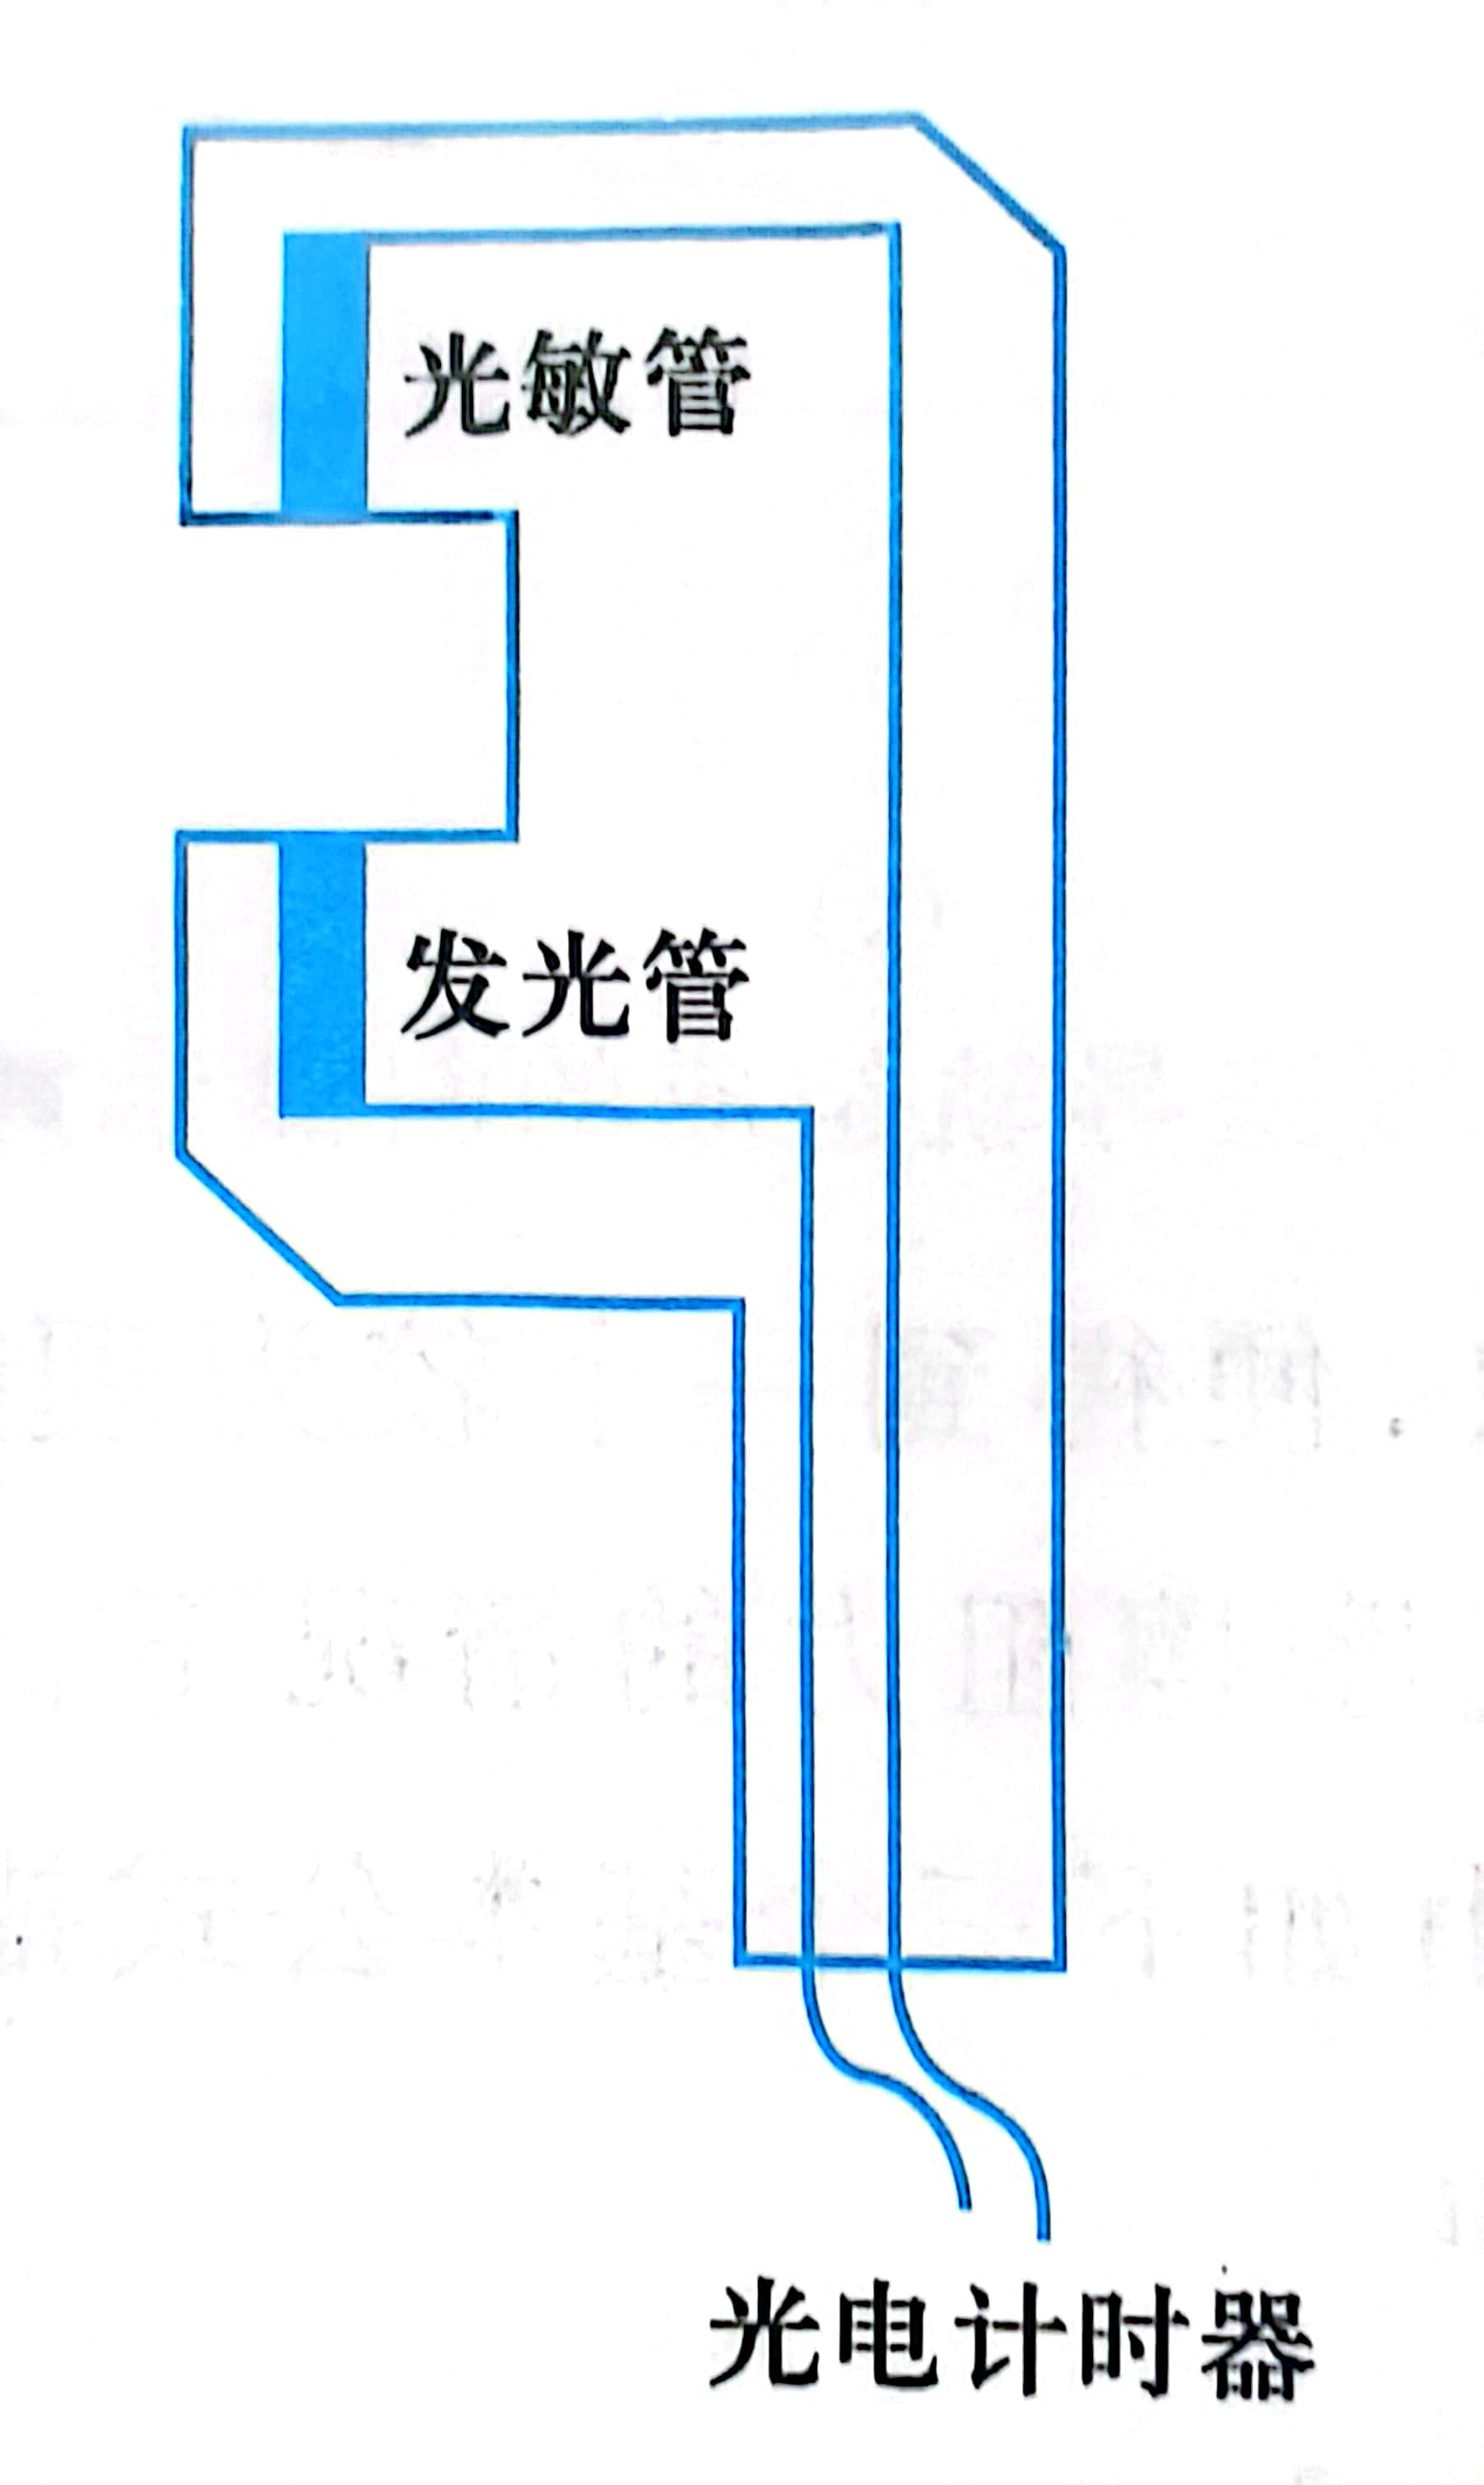
\includegraphics[height=0.2\textheight,width=0.2\textwidth]{guangdianmen.jpg}
    \caption{光电门结构示意图}\label{guangdianmen}
  \end{figure}

  光电计时系统由计时器和两个光电门组成,光电门的结构如图\ref{guangdianmen}所示,U形挡光片的结构如图\ref{dangguangpian}所示。

  光电门由红外发光二极管和光敏管组成。当U形挡光片经过光电门时,端面“1”将遮挡住发光二极管发出的光,
  进而使得光敏管接收不到红外线,这时光电门将发出开始计时的信号;当U形挡光片的端面“3”通过光电门时,
  又一次使光电门的光敏管接收不到红外线,从而发出停止计时的信号。

  \begin{figure}[H]
    \centering
    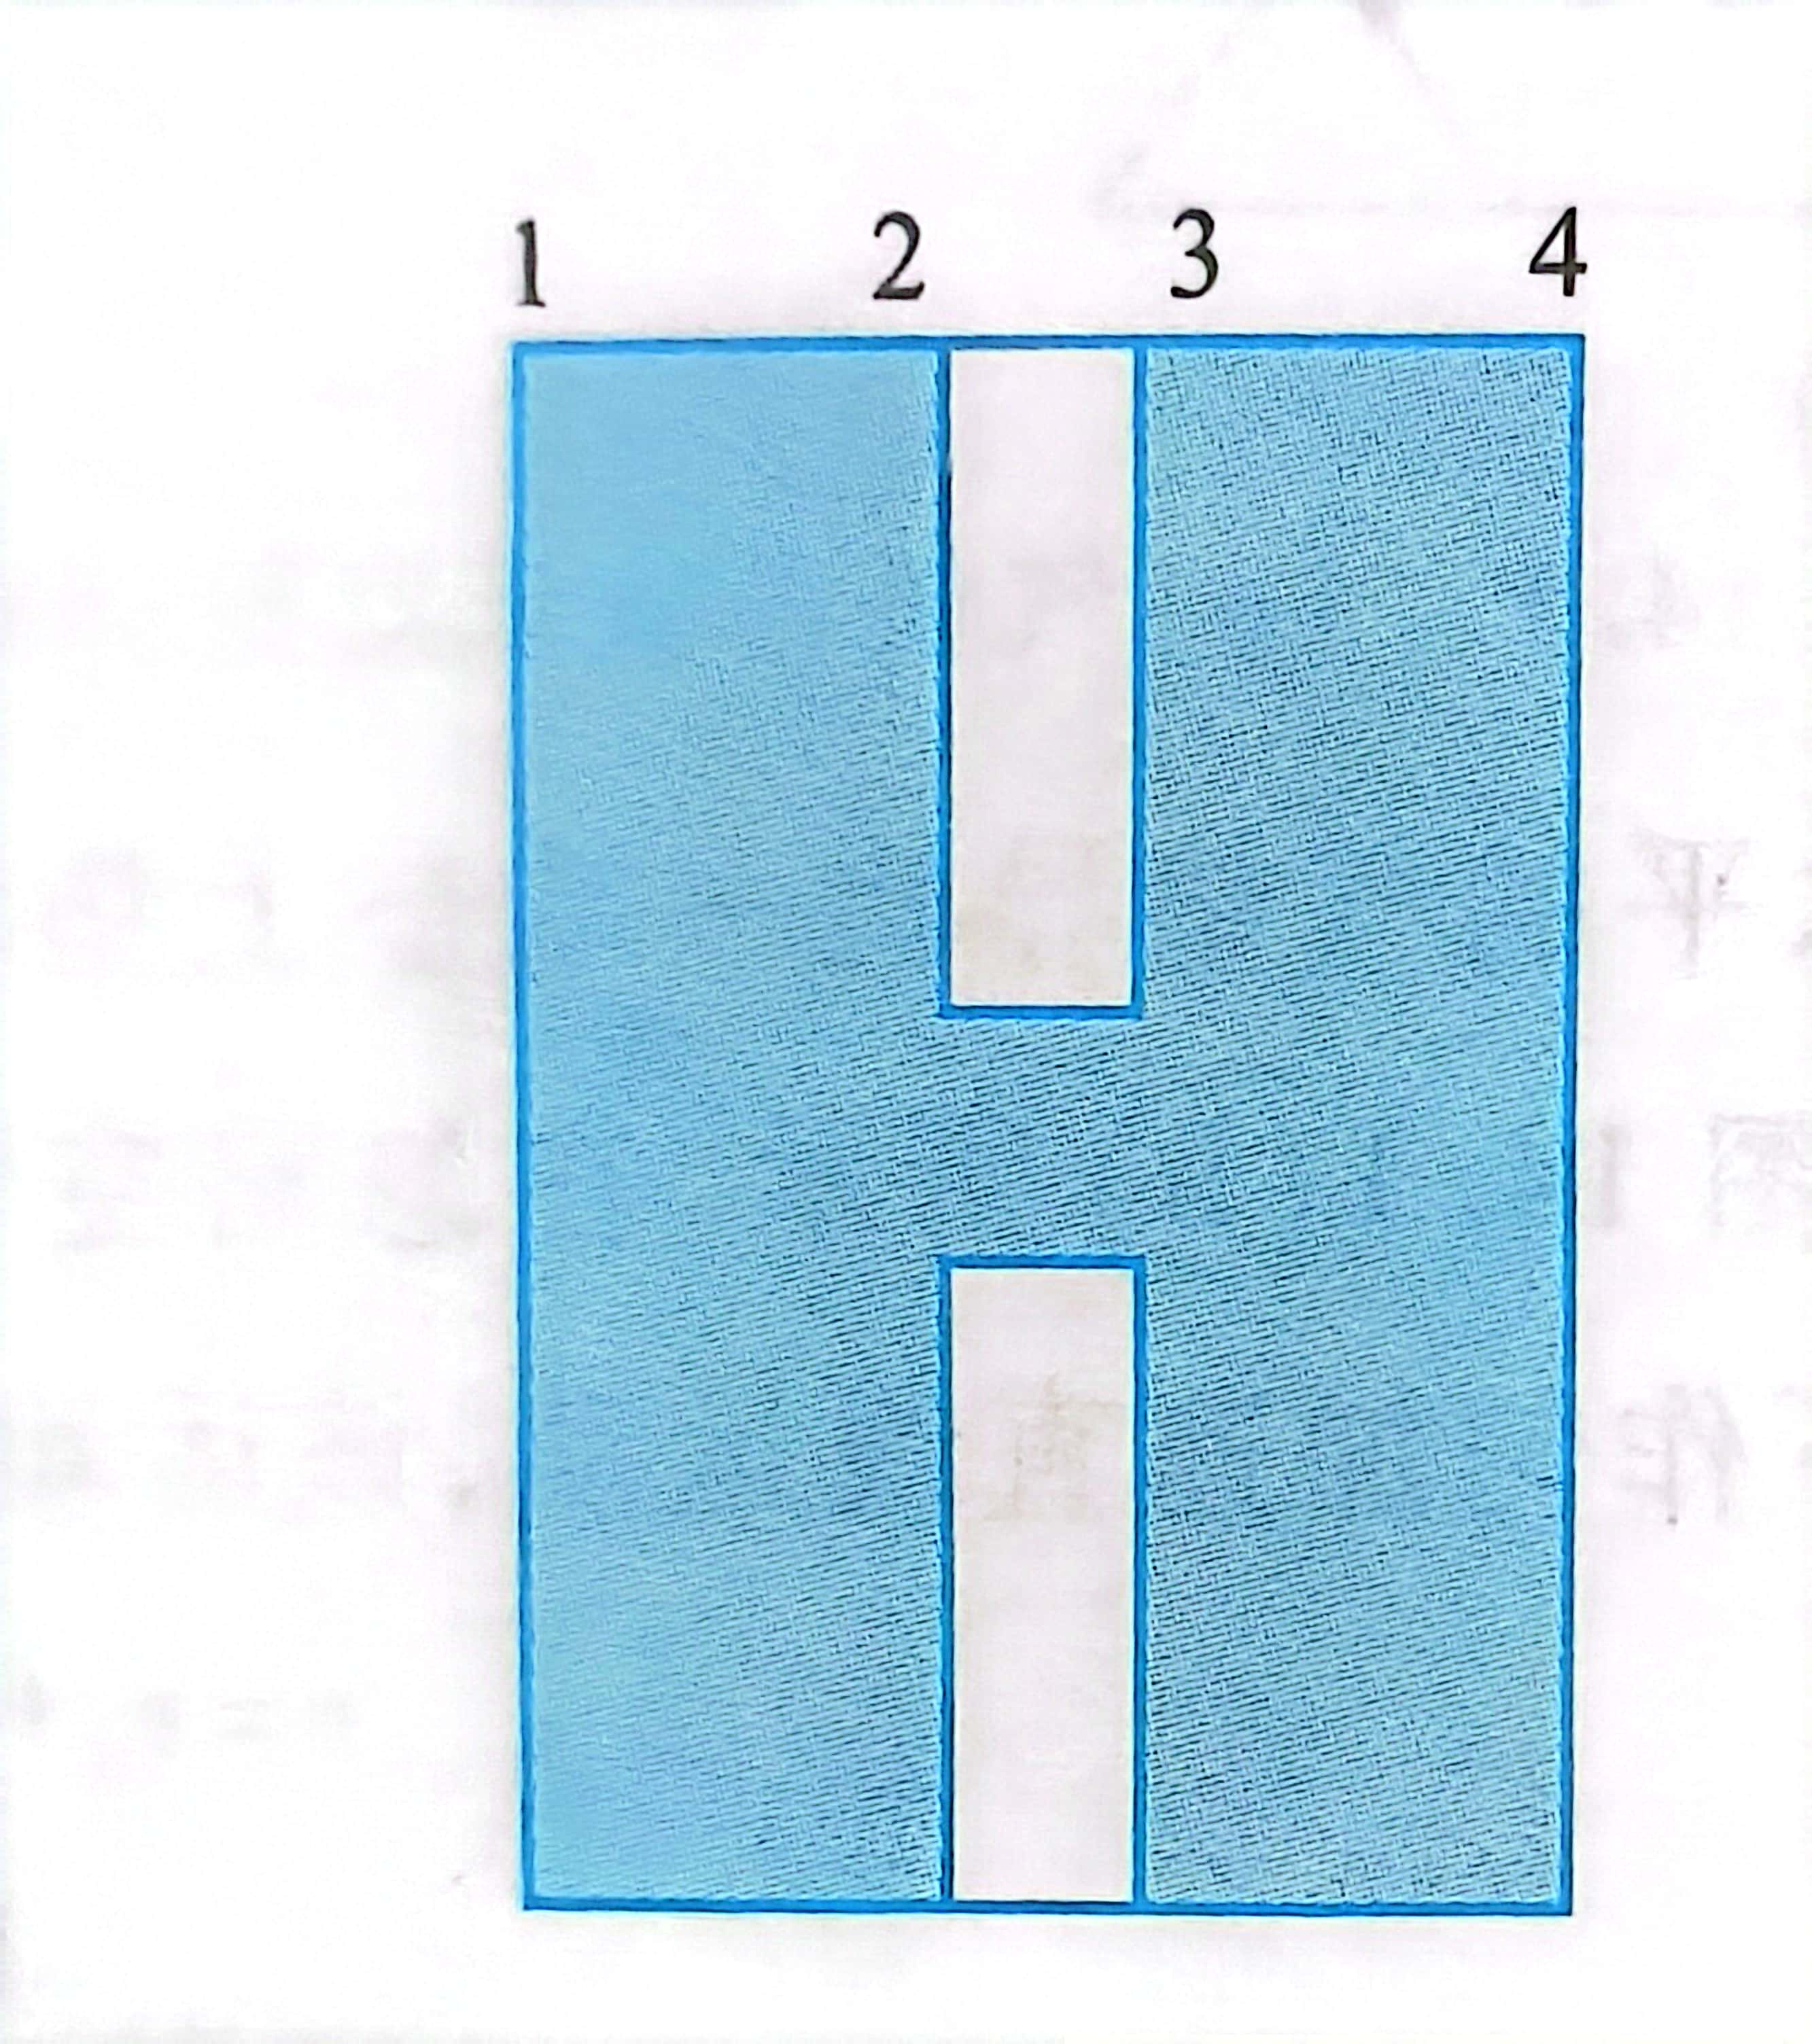
\includegraphics[height=0.2\textheight,width=0.3\textwidth]{dangguangpian.jpg}
    \caption{挡光片示意图}\label{dangguangpian}
  \end{figure}

  如果计时器获得第一次挡光到第二次挡光之间的时间为$\Delta t$,且挡光片端面1和3之间的距离为$\Delta s$,
  于是挡光片经过光电门处的平均速度可以使用式\ref{pingjunsudu}进行计算:
  
  \begin{equation}\label{pingjunsudu}
    \overline{v} = \frac{\Delta s}{\Delta t}
  \end{equation}

  在实验中,我们将该平均速度作为滑块通过光电门时的瞬时速度,计时器经过设定后,可以直接输出该速度的值。

  随后把两个光电门固定在导轨的适当位置上,并按规定和计时器连接好。
  接通计时器电源,调整计时器,使计时器输出速度值,用小纸片进行挡光试验,检查光电门和计时器是否正常工作。

  将挡光片固定在滑块上,先接通导轨上的气源,后将滑块放置导轨上,并调节滑块上的挡光片和光电门的相对位置,挡光片随滑块运动经过光电门时能实现自动挡光计时。

  \subsection{将导轨调节至水平状态}
  导轨一端下面有两个并排的底脚调节螺丝,用于调节导轨的横向水平(此项工作一般在实验室事先完成调节);
  另一端的单个螺丝用来调节导轨的纵向水平。

  \noindent(1)首先进行静态调节:通气源,滑块静止置于导轨上某处,放手时观察滑块的运动状况。如往左运动,表示右高左低,
  调节底脚螺丝,反复多次,直至滑块保持不动,或稍有移动但无一定方向性为止,应选择多个位置试验。

  \noindent(2)其次进行动态调节:如果导轨已调平,以一定初速度发射滑块,
  滑块应当作匀速直线运动,即滑块(实际是挡光片的宽度)通过两光电门的速度v1和v2近似相等。反复调节底脚螺丝,直到v1和v2相差不超过5\%。
  
  \subsection{在倾斜导轨上测量并绘制v-s图,求加速度a}
  将厚度h>3cm的垫块置于单个底脚调节螺丝下,光电门$I$置于离顶端约50cm处的$A_{0}$位置。

  光电门II依次置于离光电门I距离为10、20、30、40、50、60cm左右处,滑块每次均从顶端P处静止释放,测出滑块经过光电门I和II时的速度,
  要求对应于同一个重复5次测量取平均值$\overline{v}$。

  绘制$v^{2}-s$图,图线若为一直线,则验证了式\ref{v2},并由斜率求加速度a由截距可求得$v_{0}^{2}$,
  再将它们分别和\ref{jiasudu}式及式\ref{v2}计算得到的加速度a和初速度$v_{0}$进行比较。

  s由导轨一侧的毫米刻度尺测量,垫块厚度h和挡光片的宽度由游标卡尺测量,斜面的长度为导轨底脚螺丝之间的距离。

  \subsection{验证牛顿第一定律}
  将两个光电门固定在导轨上较远的距离(s>60 cm),光电计时器选择输出加速度的功能。

  保持两个光电门之间的距离不变,依次改变垫块的高度h(不少于5次)。在不同的高度h下,保持滑块都从同一位置释放。要求同一h下,重复5次测量滑块滑下的加速度并求平均值a。

  绘制a-h图,若为一直线,再线性外推至h=0时的情况,来验证牛顿第一定律。
\newpage

\section{实验原始数据}
\begin{figure}[H]
  \centering
  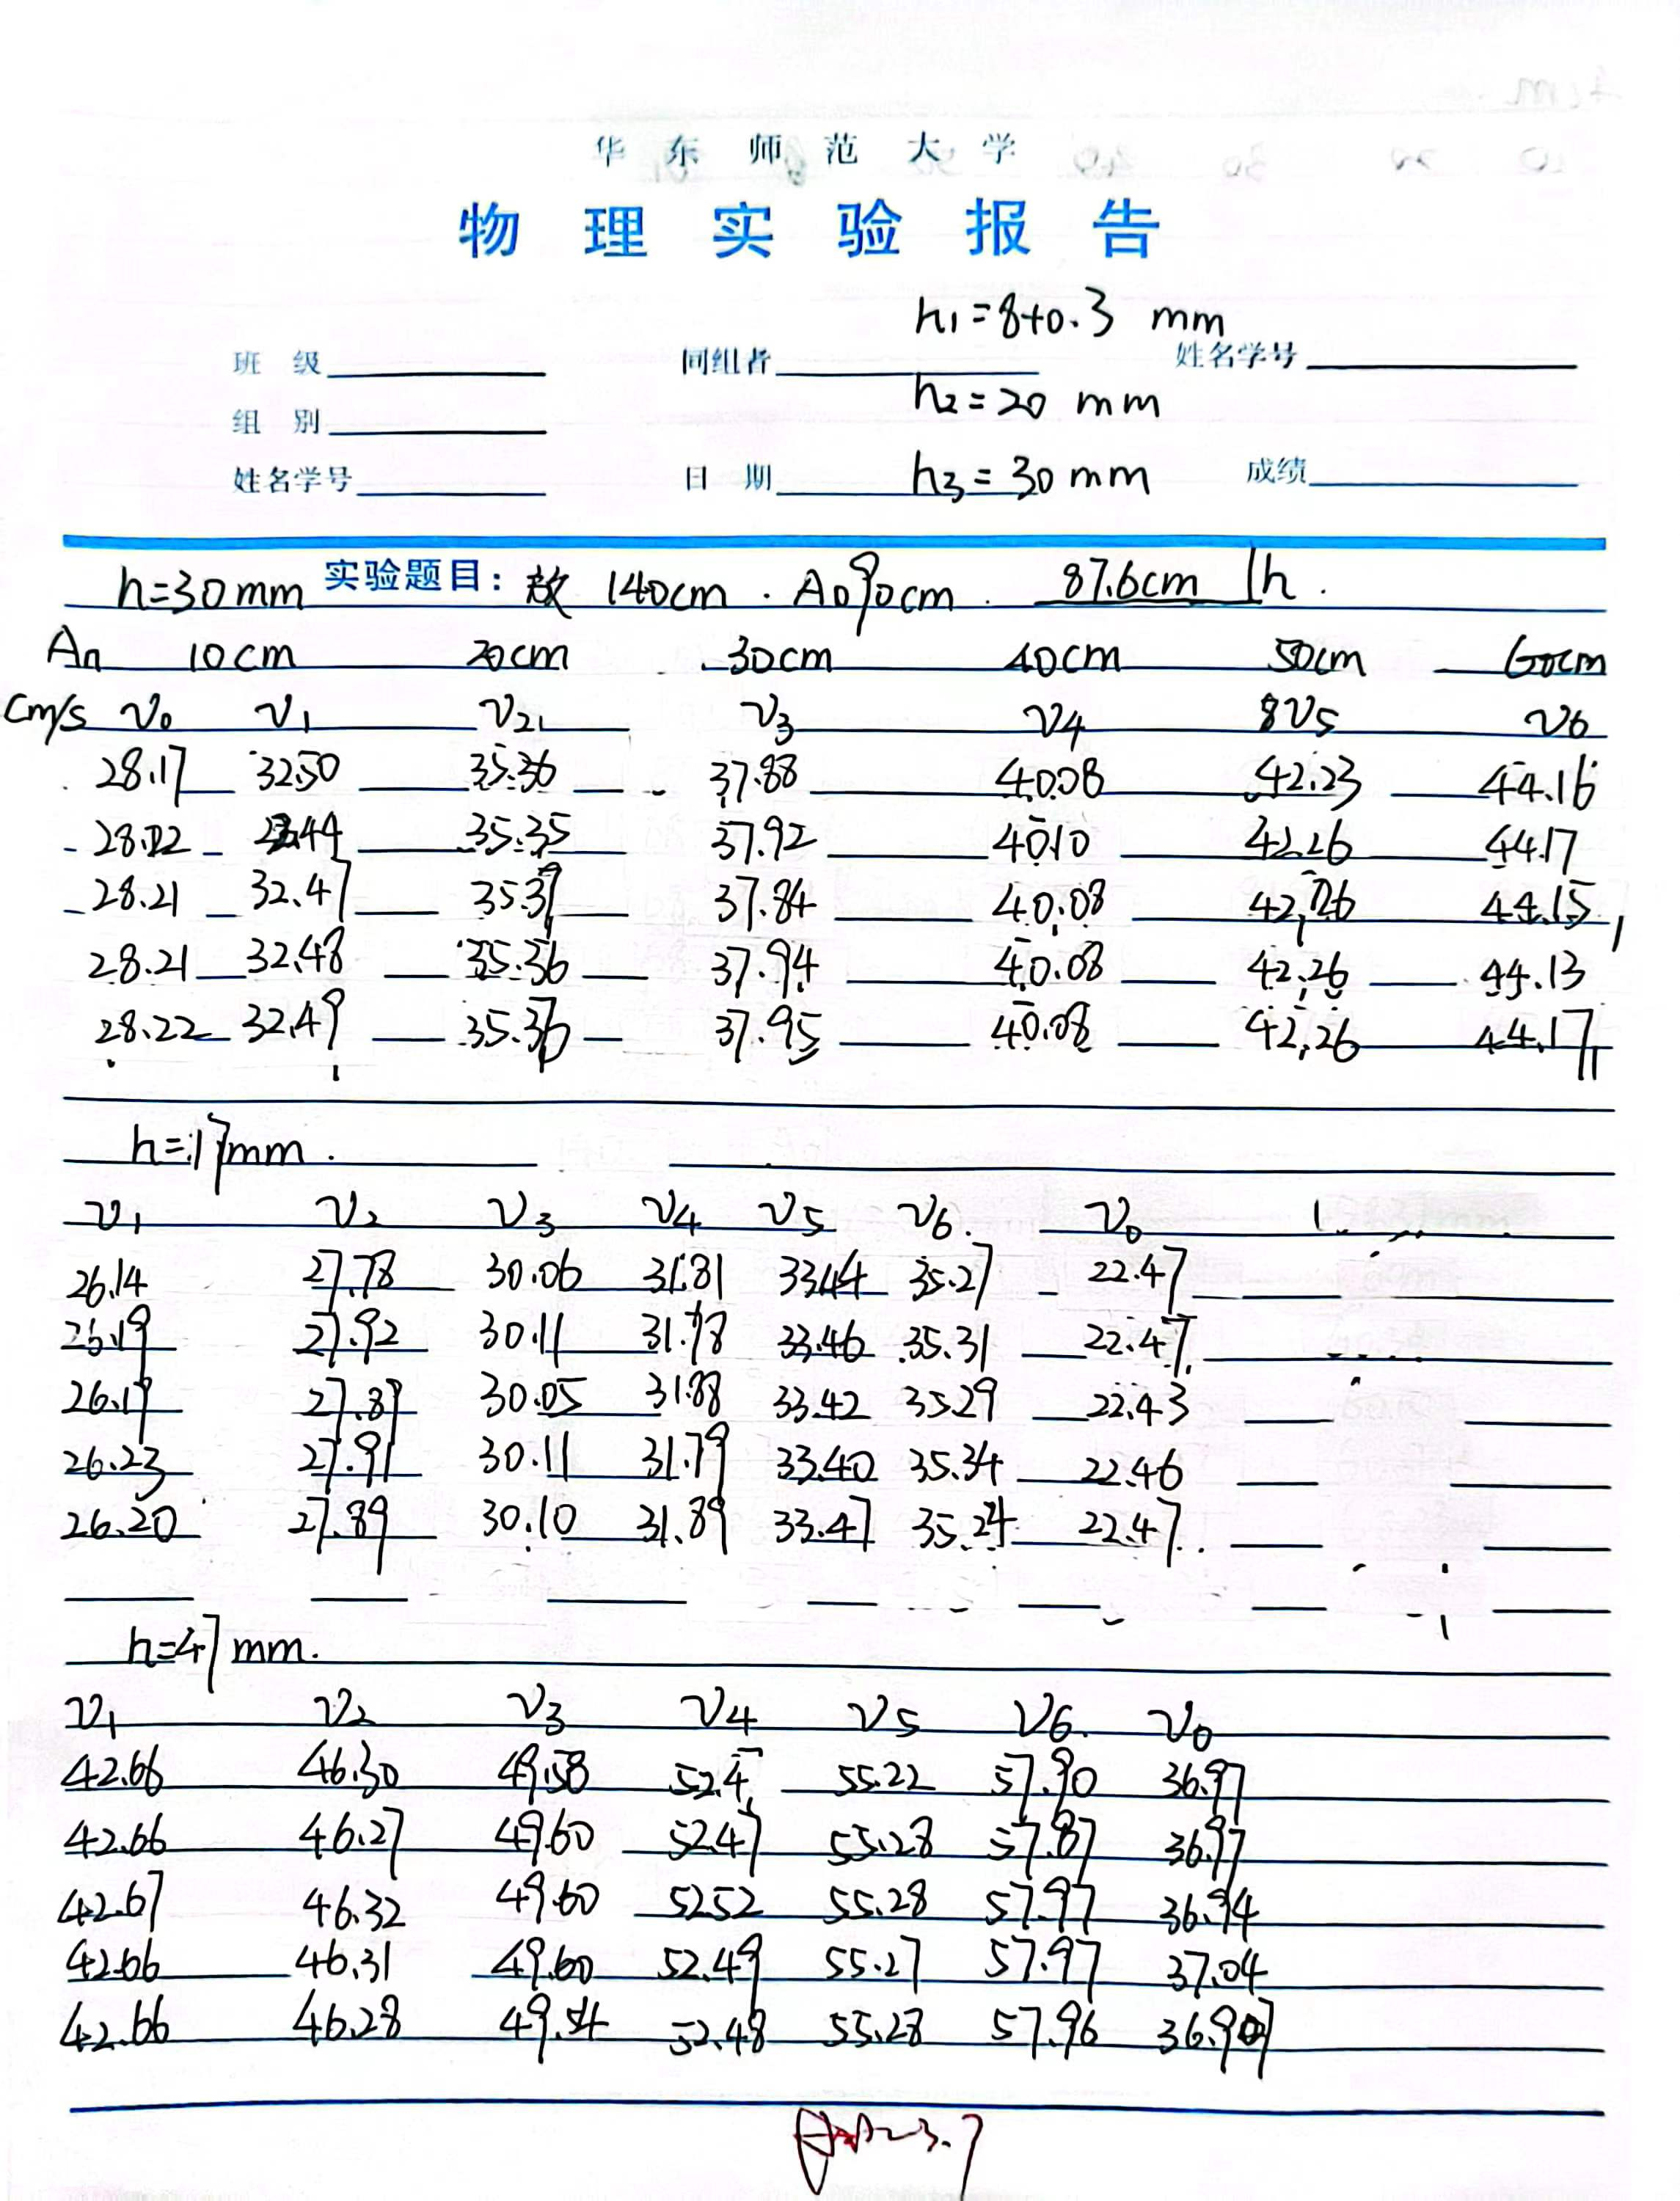
\includegraphics[height=0.8\textheight,width=1\textwidth]{yuanshishujv.jpg}
  \caption{实验原始数据1}\label{yuanshishujv}
\end{figure}
\newpage
\begin{figure}[H]
  \centering
  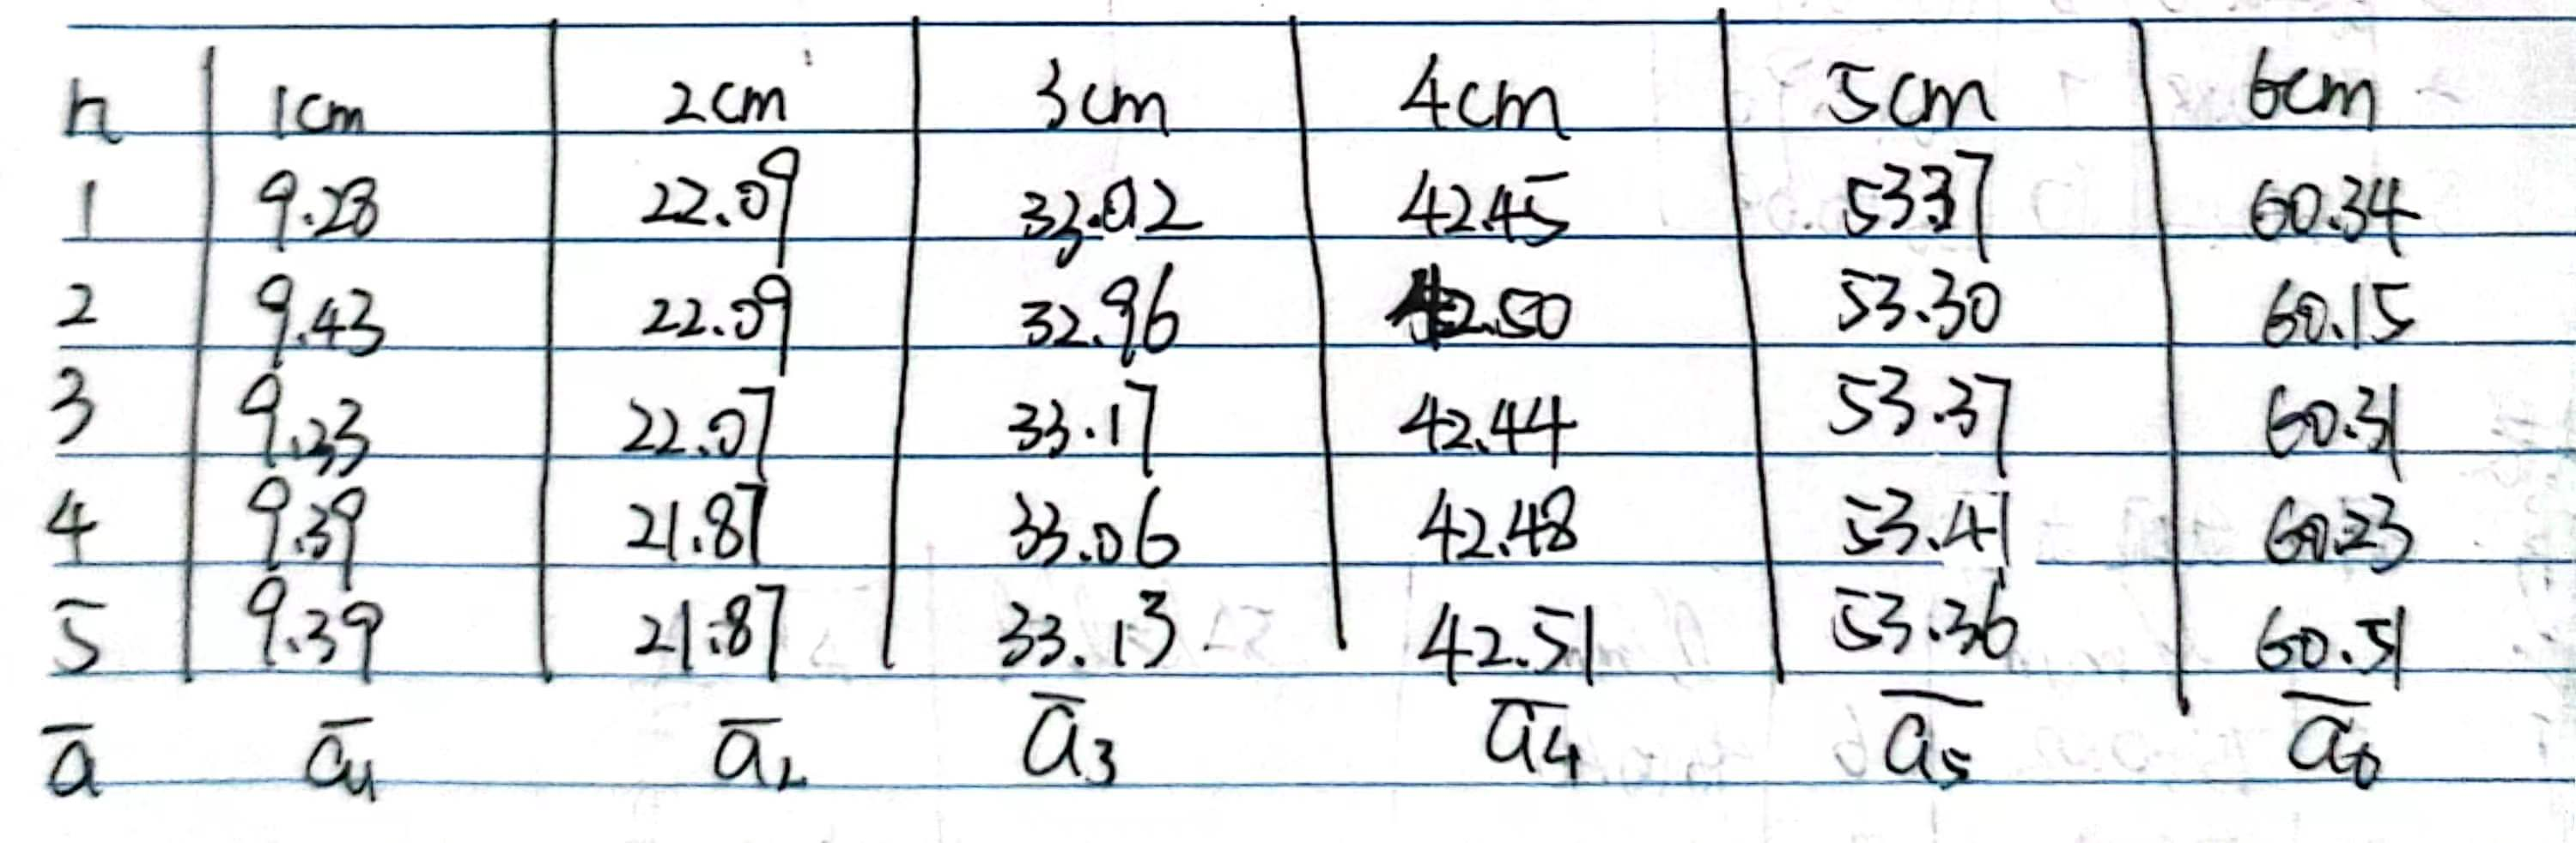
\includegraphics[height=0.3\textheight,width=1\textwidth]{yuanshishujv2.jpg}
  \caption{实验原始数据2}\label{yuanshishujv2}
\end{figure}
\newpage

\section{实验数据处理}
  \subsection{总体数据展示}
  最终得到的实验数据如图\ref{shujv}所示。
  \begin{figure}[H]
    \centering
    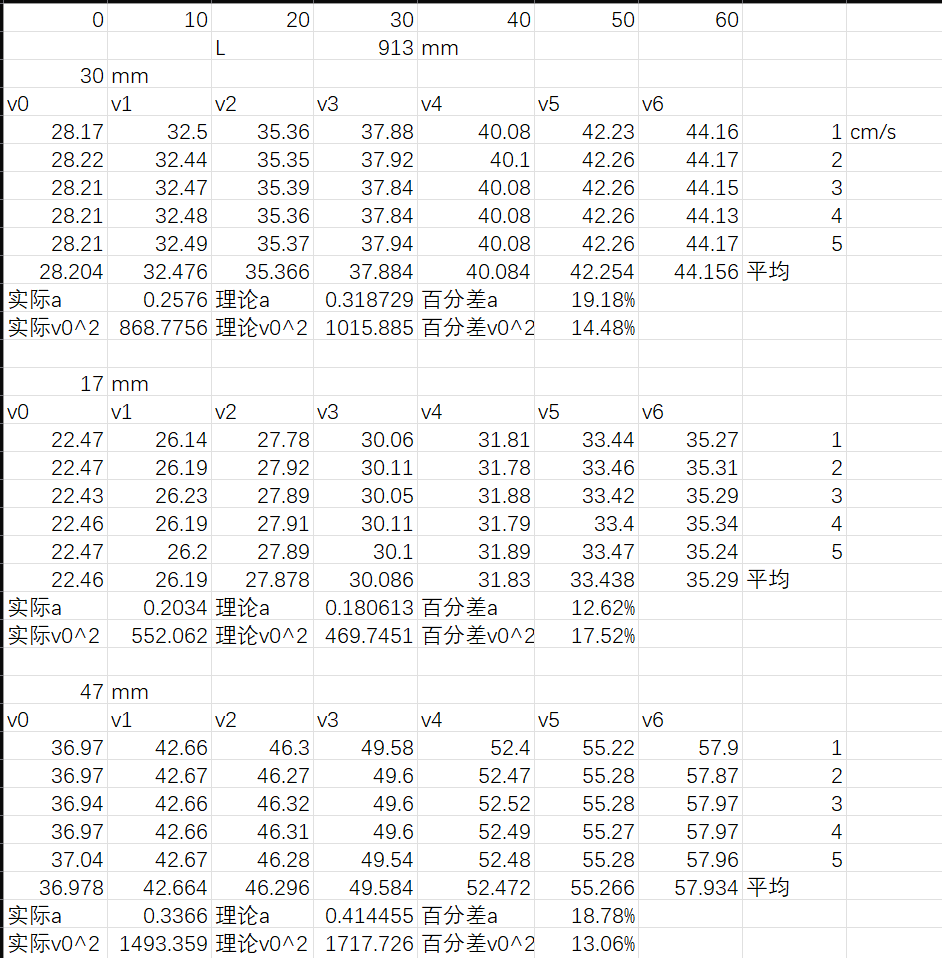
\includegraphics[height=0.7\textheight,width=1\textwidth]{zongtu.png}
    \caption{实验数据}\label{shujv}
  \end{figure}  
  \newpage

  实验得到的数据图如图\ref{zuotu}
  \begin{figure}[H]
    \centering
    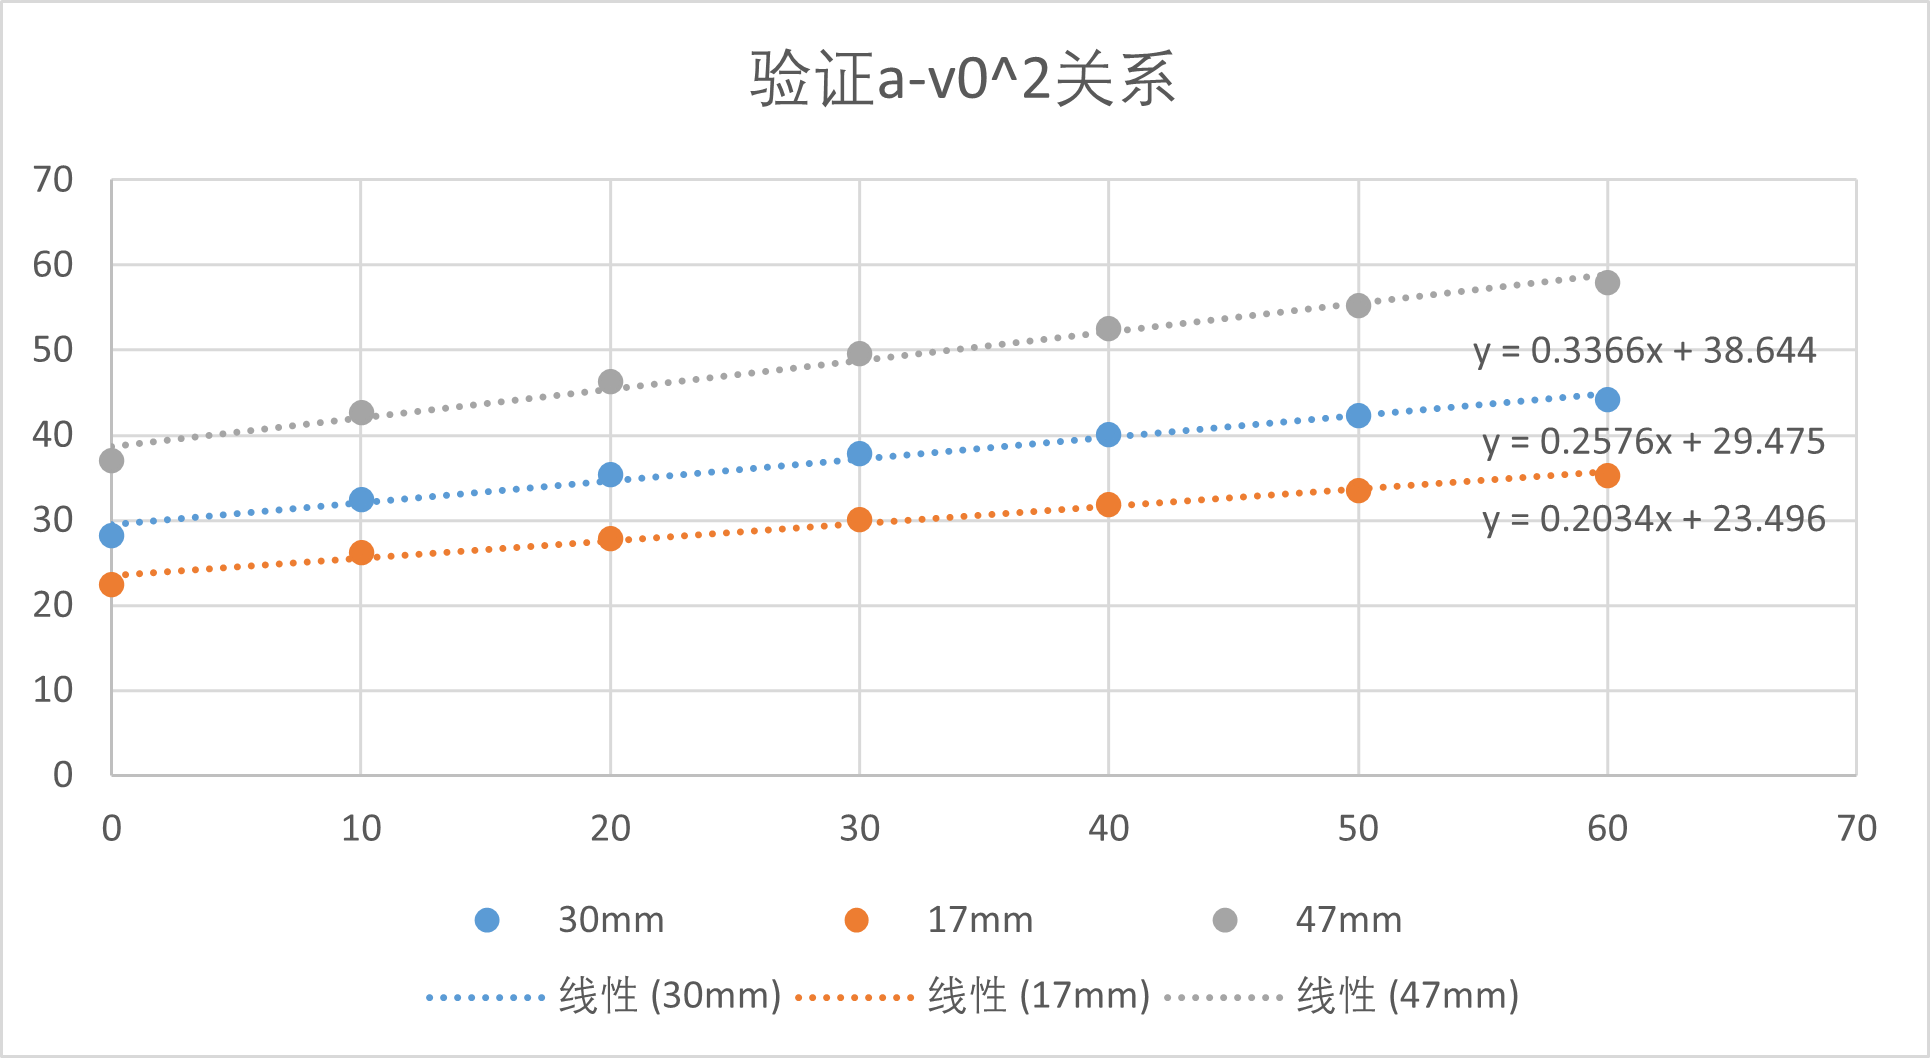
\includegraphics[height=0.35\textheight,width=0.8\textwidth]{zuotu.png}
    \caption{实验数据作图}\label{zuotu}
  \end{figure}
  实验中验证牛顿第一定律的图像如图\ref{niuyi}
  \begin{figure}[H]
    \centering
    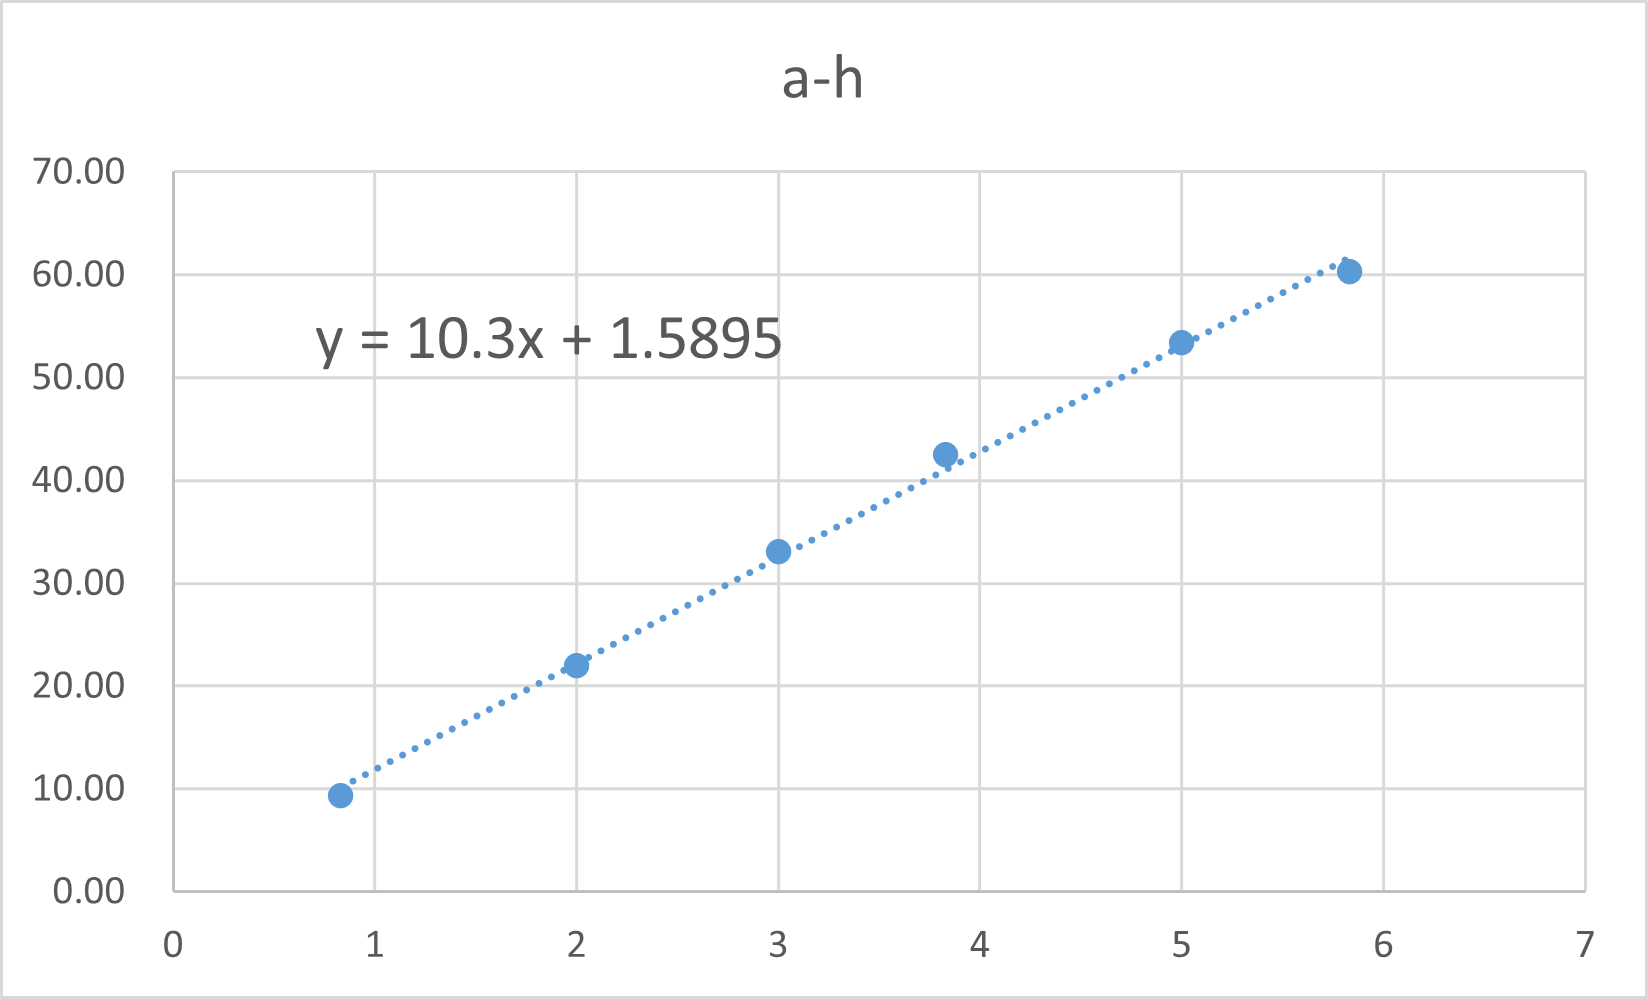
\includegraphics[height=0.35\textheight,width=0.8\textwidth]{yanzhenniuyi.png}
    \caption{实验数据作图}\label{niuyi}
  \end{figure}
  \newpage

  \subsection{不同倾斜角度下实验计算}
  \subsubsection{17mm高度}
  实验得到的数据如图\ref{17mm}。
  \begin{figure}[H]
    \centering
    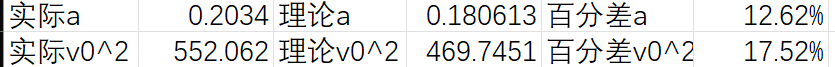
\includegraphics[height=0.1\textheight,width=0.85\textwidth]{17mm.png}
    \caption{17mm高度实验数据作图}\label{17mm}
  \end{figure}
  最终得到的a的百分差为12.62\%,而$v_{0}^{2}$的误差为17.52\%。

  \subsubsection{30mm高度}
  实验得到的数据如图\ref{30mm}。
  \begin{figure}[H]
    \centering
    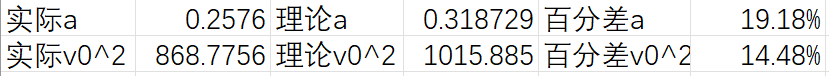
\includegraphics[height=0.1\textheight,width=0.85\textwidth]{30mm.png}
    \caption{30mm高度实验数据作图}\label{30mm}
  \end{figure}
  最终得到的a的百分差为19.18\%,而$v_{0}^{2}$的误差为14.48\%。

  \subsubsection{47mm高度}
  实验得到的数据如图\ref{47mm}。
  \begin{figure}[H]
    \centering
    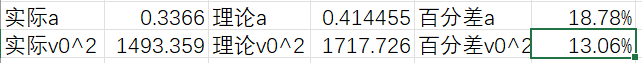
\includegraphics[height=0.1\textheight,width=0.85\textwidth]{47mm.png}
    \caption{47mm高度实验数据作图}\label{47mm}
  \end{figure}
  最终得到的a的百分差为18.78\%,而$v_{0}^{2}$的误差为13.06\%。

  \subsection{误差分析}
  实验最终得到的数据的误差都比较大。可能存在的原因如下:

  \noindent (1) \quad 实验中使用的气垫导轨其实是存在阻力的。当倾斜角度逐渐升高的时候,喷气口产生的阻力越大导致误差越大。

  \noindent (2) \quad 调节水平后放置增高块的时候触碰调节高度的旋钮导致在水平的时候不能平衡出现问题。

  \noindent (3) \quad 释放滑块的时候不是静止释放,导致带有一定初速度释放产生误差。

    
\section{思考题}
  \subsection{思考题1}
  使用两种方法进行水平的测定更加准确。防止轨道有一定摩擦导致某种方案不那么适用。
  \subsection{思考题2} 
  不能直接得出,可能是吹气的气垫吹气量不同导致受到向下的力的作用。
  可以通过检测吹气量得出。而且还可能是在一开始具有初速度受到向下的力的作用。
  \subsection{思考题3}
  光电门之间的距离越大,测得的加速度值越接近真值。
\newpage

\section{实验中个人的思考与感想}
  \subsection{对于实验个人观点}
  实验的原理非常简单,就是验证的实验。实验中的操作也比较简单,主要难点集中在如何将导轨调节
  水平减少误差和从静止释放滑块。但是实验结果却显示似乎实验中的误差还是很大的。当然,
  在之前的自主实验探索中我也在相同设备上进行了阻尼运动的实验,所以其实气垫导轨也是有阻力的。

  实验之前也做过,但是数据比这次要好看很多,误差都在10\%以内。所以实验也有运气成分吧。但是之前
  的实验中没有进行不同高度的多次测量,所以一定程度上存在幸存者偏差。
  \subsection{实验中的总结}
  实验测量了速度和运动距离以及倾斜角度的关系,计算了$a - v_{0}^2$的关系,计算了理论与实验的误差。
  误差较大。并且验证了牛顿第一定律。
\end{document}